\section{Cronograma}
\justifying
Devido à pandemia e a consequente incerteza no calendário acadêmico da UFMG em 2020, o cronograma foi divido por semanas e sem datas específicas. Portanto, considerou-se que os 2 semestres que consistirão no desenvolvimento desse projeto terão, aproximadamente, 38 semanas.

As tarefas desse projeto foram dividas em três grupos: Desenvolvimento, Relatório e Modelagem. O grupo  Desenvolvimento engloba as atividades relacionadas à programação e modelagem de banco de dados. Relatório são aquelas atividades relacionadas ao desenvolvimento do relatório do projeto e modelagem é a pesquisa e definição da metodologia implementada.

    \begin{figure}[H]
    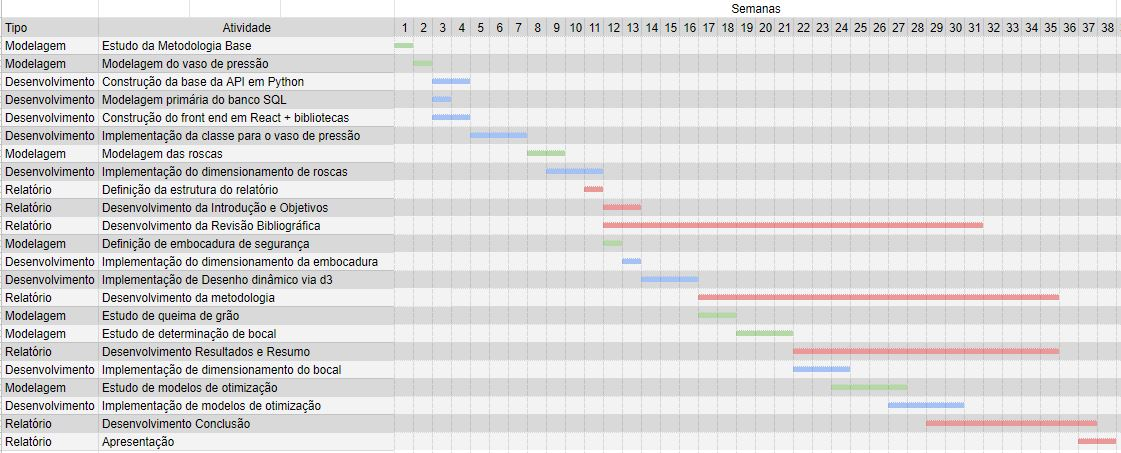
\includegraphics[scale=0.5]{Imagens/Cronograma.jpg}
    \centering
    \caption{Cronograma do Projeto}
    \label{Schedule}
    \end{figure}